%==============================================================================
%  ENGR 2405 - Electrical Circuits I
%  Lab 8 - Transient Response II
%==============================================================================
\documentclass[11pt]{article}

%------------------------- Packages -------------------------------------------
\usepackage[utf8]{inputenc}
\usepackage[T1]{fontenc}
\usepackage[margin=1in]{geometry}
\usepackage{amsmath,amssymb}
\usepackage{graphicx}
\usepackage{float}
\usepackage{booktabs}
\usepackage{siunitx}
\usepackage{listings}
\usepackage{xcolor}
\usepackage{caption}
\usepackage[hidelinks]{hyperref}
\usepackage{titlesec}

%------------------------- Section styling ------------------------------------
\titleformat{\section}{\Large\bfseries}{}{0pt}{}
\titlespacing*{\section}{0pt}{1.4em}{0.6em}

%------------------------- Code listing style ---------------------------------
\definecolor{codebg}{RGB}{245,245,245}
\definecolor{codecomment}{RGB}{0,128,0}
\definecolor{codekw}{RGB}{0,0,180}
\lstset{
    backgroundcolor=\color{codebg},
    basicstyle=\ttfamily\small,
    breaklines=true,
    frame=single,
    framesep=4pt,
    keywordstyle=\color{codekw}\bfseries,
    commentstyle=\color{codecomment}\itshape,
    showstringspaces=false,
    captionpos=b,
    tabsize=2,
}
\definecolor{codestr}{RGB}{163,21,21}
\definecolor{codenum}{RGB}{120,120,120}

% --- LTSpice netlist ----------------------------------------------------------
\lstdefinelanguage{LTspice}{
    morekeywords={
        .tran,.op,.dc,.ac,.step,.param,.model,.lib,.include,.inc,
        .meas,.measure,.save,.backanno,.end,.ends,.subckt,.global,
        .ic,.nodeset,.options,.option,.func,.temp,.four,.noise,.tf
    },
    sensitive=false,
    morecomment=[l]{*},
    morecomment=[l]{;},
    morestring=[b]",
}
\lstdefinestyle{netlist}{
    language=LTspice,
    keywordstyle=\color{codekw}\bfseries,
    basicstyle=\ttfamily\small,
}

% --- SciLab (custom: listings has no built-in SciLab language) --------------
\lstdefinelanguage{Scilab}{
    morekeywords={
        function,endfunction,if,then,else,elseif,end,for,while,do,
        select,case,break,continue,return,clc,clear,disp,mprintf,
        printf,zeros,ones,eye,linspace,inv,det,sum,length,size,abs,
        sqrt,real,imag,exp,sin,cos,tan,plot,plot2d,xlabel,ylabel,
        title,legend,xgrid,scf,clf,poly,roots,find,pause,error,warning
    },
    sensitive=true,
    morecomment=[l]{//},
    morecomment=[s]{/*}{*/},
    morestring=[b]",
    morestring=[b]',
}
\lstdefinestyle{scilab}{
    language=Scilab,
    stringstyle=\color{codestr},
}

%==============================================================================
\begin{document}

%------------------------- Title block ----------------------------------------
\begin{center}
    {\LARGE\bfseries Lab 8 - Transient Response II}\\[0.8em]
    {\large Abdon Morales}\\[0.3em]
    {\large \today}
\end{center}
\vspace{1em}

%------------------------------------------------------------------------------
\section*{Description}

In this lab we study the transient response of a second-order circuit built from
an op-amp, two resistors, and two capacitors. The circuit is a unity-gain
Sallen-Key low-pass filter, which lets us synthesize a second-order response
without an inductor. We design the circuit three ways so that it produces a
critically damped, an overdamped, and an underdamped step response, all at a
resonant frequency near \SI{1}{\kilo\hertz}. For each case we solve the governing
differential equation by hand, simulate the circuit in KiCad, and measure the
step response on the bench with a \SI{100}{\hertz}, \SI{2}{\volt} peak-to-peak
square wave as the input. We then compare the three sets of results.

%------------------------------------------------------------------------------
\section*{Procedure}

\begin{enumerate}
    \item We designed three Sallen-Key circuits in KiCad using the design
    equations for $\alpha$, $\omega_0$, and $Q$, choosing standard component
    values that place each circuit in one of the three damping regimes while
    keeping $f_0$ near \SI{1}{\kilo\hertz}.
    \item We drove each simulated circuit with a \SI{100}{\hertz},
    \SI{2}{\volt} peak-to-peak square wave and recorded the transient response.
    \item We built each circuit on the XK700 trainer using a 741 op-amp. Where a
    designed resistor or capacitor value was not available in the lab kit, we
    substituted the nearest stocked part, so the built values differ from the
    design table (see the Measurements section).
    \item We used the function generator on the XK700 to apply a \SI{100}{\hertz},
    \SI{2}{\volt} peak-to-peak square wave to the input.
    \item We displayed the input on CH1 and the output on CH2 of the oscilloscope
    and recorded the waveforms for each of the three cases.
\end{enumerate}

%------------------------------------------------------------------------------
\section*{Calculations}

\textbf{Governing equation.} Applying KCL at the two internal nodes of the
Sallen-Key circuit and combining the results gives the second-order differential
equation for the output:
\[
    R_1 C_1 R_2 C_2 \, \frac{d^2 V_{out}}{dt^2}
    + (R_1 + R_2) C_2 \, \frac{d V_{out}}{dt}
    + V_{out} = V_{in}.
\]
Dividing through by $R_1 C_1 R_2 C_2$ puts this in standard form,
\[
    \frac{d^2 V_{out}}{dt^2} + 2\alpha \frac{d V_{out}}{dt} + \omega_0^2 V_{out}
    = \omega_0^2 V_{in},
\]
where the damping factor and resonant frequency for this topology are
\[
    2\alpha = \frac{1}{R_{eq} C_1}, \qquad
    \omega_0^2 = \frac{1}{R_1 C_1 R_2 C_2}, \qquad
    \frac{1}{R_{eq}} = \frac{1}{R_1} + \frac{1}{R_2}.
\]
The quality factor is $Q = \omega_0 / (2\alpha)$, so $Q = \tfrac{1}{2}$ separates
the overdamped ($Q < \tfrac{1}{2}$) and underdamped ($Q > \tfrac{1}{2}$) cases.
At DC the capacitors are open and the follower passes the input straight through,
so the DC gain is one and the particular solution is $V_{out} = V_{in}$.

\textbf{Component selection.} We fixed the geometric-mean time constant to hold
$\omega_0$ near $2000\pi\ \si{\radian\per\second}$ and adjusted the component
ratios to set $Q$. For the critically damped case we used equal resistors and
equal capacitors, which forces $Q = \tfrac{1}{2}$ exactly. For the overdamped
case we kept the capacitors equal and split the resistors, which drops $Q$ below
$\tfrac{1}{2}$ while keeping $\sqrt{R_1 R_2}$ fixed. For the underdamped case we
kept the resistors equal and raised $C_1$ above $C_2$, which pushes $Q$ above
$\tfrac{1}{2}$. Table~\ref{tab:design} lists the three designs and the resulting
parameters.

\begin{table}[H]
    \centering
    \caption{Component values and derived parameters for the three cases.}
    \label{tab:design}
    \begin{tabular}{lccccccc}
        \toprule
        Case & $R_1$ & $R_2$ & $C_1$ & $C_2$ & $Q$ & $f_0$ (Hz) & $\alpha$ (s$^{-1}$) \\
        \midrule
        Critically damped & \SI{16}{\kilo\ohm} & \SI{16}{\kilo\ohm} & \SI{10}{\nano\farad} & \SI{10}{\nano\farad} & 0.500 & 994.7 & 6250 \\
        Overdamped        & \SI{47}{\kilo\ohm} & \SI{5.6}{\kilo\ohm} & \SI{10}{\nano\farad} & \SI{10}{\nano\farad} & 0.308 & 981.0 & 9992 \\
        Underdamped       & \SI{10}{\kilo\ohm} & \SI{10}{\kilo\ohm} & \SI{22}{\nano\farad} & \SI{10}{\nano\farad} & 0.742 & 1073 & 4545 \\
        \bottomrule
    \end{tabular}
\end{table}

\textbf{Step response.} The square-wave input steps by $\Delta V = \SI{2}{\volt}$
on each edge. Since the circuit fully settles in well under the \SI{5}{\milli\second}
half-period, every edge produces a complete step response. Both capacitor voltages
are continuous through an edge and the circuit carries no DC current in steady
state, so the initial conditions after a step are $V_{out}(0) = V_0$ and
$\dot{V}_{out}(0) = 0$, where $V_0$ is the level before the edge. Writing the
output as $V_{out}(t) = V_0 + \Delta V\, g(t)$, the normalized response $g(t)$ rises
from $0$ to $1$ and is found below for each case.

\emph{Critically damped} ($\alpha = \omega_0 = 6250\ \si{\per\second}$, repeated
root $s = -6250\ \si{\per\second}$):
\[
    g(t) = 1 - (1 + \alpha t)\, e^{-\alpha t}.
\]
This rises to the final value in the shortest time possible without overshoot,
with a time constant $1/\alpha = \SI{160}{\micro\second}$.

\emph{Overdamped} (real roots $s_1 = -2128\ \si{\per\second}$,
$s_2 = -17857\ \si{\per\second}$):
\[
    g(t) = 1 + \frac{s_2\, e^{s_1 t} - s_1\, e^{s_2 t}}{s_1 - s_2}
         = 1 - 1.135\, e^{-2128\,t} + 0.135\, e^{-17857\,t}.
\]
The slow root ($\tau_1 = \SI{470}{\micro\second}$) dominates, so the output climbs
to its final value slowly and without overshoot.

\emph{Underdamped} (complex roots $s = -4545 \pm j\,4979\ \si{\per\second}$,
$\omega_d = 4979\ \si{\radian\per\second}$, $f_d = \SI{792}{\hertz}$):
\[
    g(t) = 1 - e^{-\alpha t}\!\left( \cos\omega_d t
           + \frac{\alpha}{\omega_d}\sin\omega_d t \right),
    \qquad \frac{\alpha}{\omega_d} = 0.913.
\]
This overshoots and rings. The predicted overshoot is
$e^{-\pi\alpha/\omega_d} = 5.7\%$ at a peak time
$t_p = \pi/\omega_d = \SI{631}{\micro\second}$.

We checked the three designs in SciLab. The script below computes $R_{eq}$,
$\omega_0$, $\alpha$, $Q$, and the characteristic-equation roots for each case
and plots the normalized step responses.

\begin{lstlisting}[style=scilab, caption={SciLab: damping parameters and step response}]
// Sallen-Key second-order step response.
// C1 = feedback cap, C2 = grounded cap.
clear; clc;

names = ["Critically damped"; "Overdamped"; "Underdamped"];
R1 = [16e3;  47e3;  10e3];    // ohms
R2 = [16e3;  5.6e3; 10e3];
C1 = [10e-9; 10e-9; 22e-9];   // farads
C2 = [10e-9; 10e-9; 10e-9];

t = linspace(0, 3e-3, 3000);
scf(0); clf();

for k = 1:3
    Req   = R1(k)*R2(k)/(R1(k)+R2(k));
    w0    = sqrt(1/(R1(k)*C1(k)*R2(k)*C2(k)));
    alpha = 1/(2*Req*C1(k));
    Q     = w0/(2*alpha);
    f0    = w0/(2*%pi);
    zeta  = alpha/w0;          // damping ratio: 1 = critical

    mprintf("\n%s\n", names(k));
    mprintf("  Req = %7.1f ohm   f0 = %7.1f Hz   Q = %5.3f\n", Req, f0, Q);
    mprintf("  w0  = %7.1f rad/s   alpha = %7.1f 1/s\n", w0, alpha);

    if abs(zeta - 1) < 1e-3 then
        mprintf("  critically damped: double root s = %8.1f 1/s\n", -alpha);
        g = 1 - (1 + alpha*t).*exp(-alpha*t);
    elseif zeta > 1 then
        s1 = -alpha + alpha*sqrt(1 - 1/zeta^2);
        s2 = -alpha - alpha*sqrt(1 - 1/zeta^2);
        mprintf("  overdamped: s1 = %8.1f   s2 = %9.1f 1/s\n", s1, s2);
        g = 1 + (s2*exp(s1*t) - s1*exp(s2*t))/(s1 - s2);
    else
        wd = w0*sqrt(1 - zeta^2);
        Mp = exp(-%pi*alpha/wd)*100;
        mprintf("  underdamped: s = -%.1f +/- j%.1f 1/s   fd = %.1f Hz\n", ...
                alpha, wd, wd/(2*%pi));
        mprintf("  overshoot = %.1f %%   tp = %.0f us\n", Mp, %pi/wd*1e6);
        g = 1 - exp(-alpha*t).*(cos(wd*t) + (alpha/wd)*sin(wd*t));
    end

    plot(t*1e3, g);
end

xlabel("Time (ms)");
ylabel("Normalized V_out");
legend(names(1), names(2), names(3), 4);
xgrid();
\end{lstlisting}

\begin{lstlisting}[caption={SciLab runtime output}]
-->exec('/mnt/c/Users/Abdon Morales/OneDrive - The University of Texas at Austin/Summer 2026/ECE 402/Lab Notes/Lab 08/lab8_calc.sce', -1)

Critically damped
  Req =  8000.0 ohm   f0 =   994.7 Hz   Q = 0.500
  w0  =  6250.0 rad/s   alpha =  6250.0 1/s
  critically damped: double root s =  -6250.0 1/s

Overdamped
  Req =  5003.8 ohm   f0 =   981.0 Hz   Q = 0.308
  w0  =  6163.9 rad/s   alpha =  9992.4 1/s
  overdamped: s1 =  -2127.7   s2 =  -17857.1 1/s

Underdamped
  Req =  5000.0 ohm   f0 =  1073.0 Hz   Q = 0.742
  w0  =  6742.0 rad/s   alpha =  4545.5 1/s
  underdamped: s = -4545.5 +/- j4979.3 1/s   fd = 792.5 Hz
  overshoot = 5.7 %   tp = 631 us

\end{lstlisting}

%------------------------------------------------------------------------------
\section*{Simulations}

We built each circuit in KiCad and simulated it with ngspice, using the built-in
op-amp model as a unity-gain buffer on \SI{\pm 15}{\volt} rails and a
\SI{100}{\hertz}, \SI{2}{\volt} peak-to-peak square wave at the input. The
netlists KiCad generated are shown below, with the transient plot following each
one.

\begin{figure}[H]
    \centering
    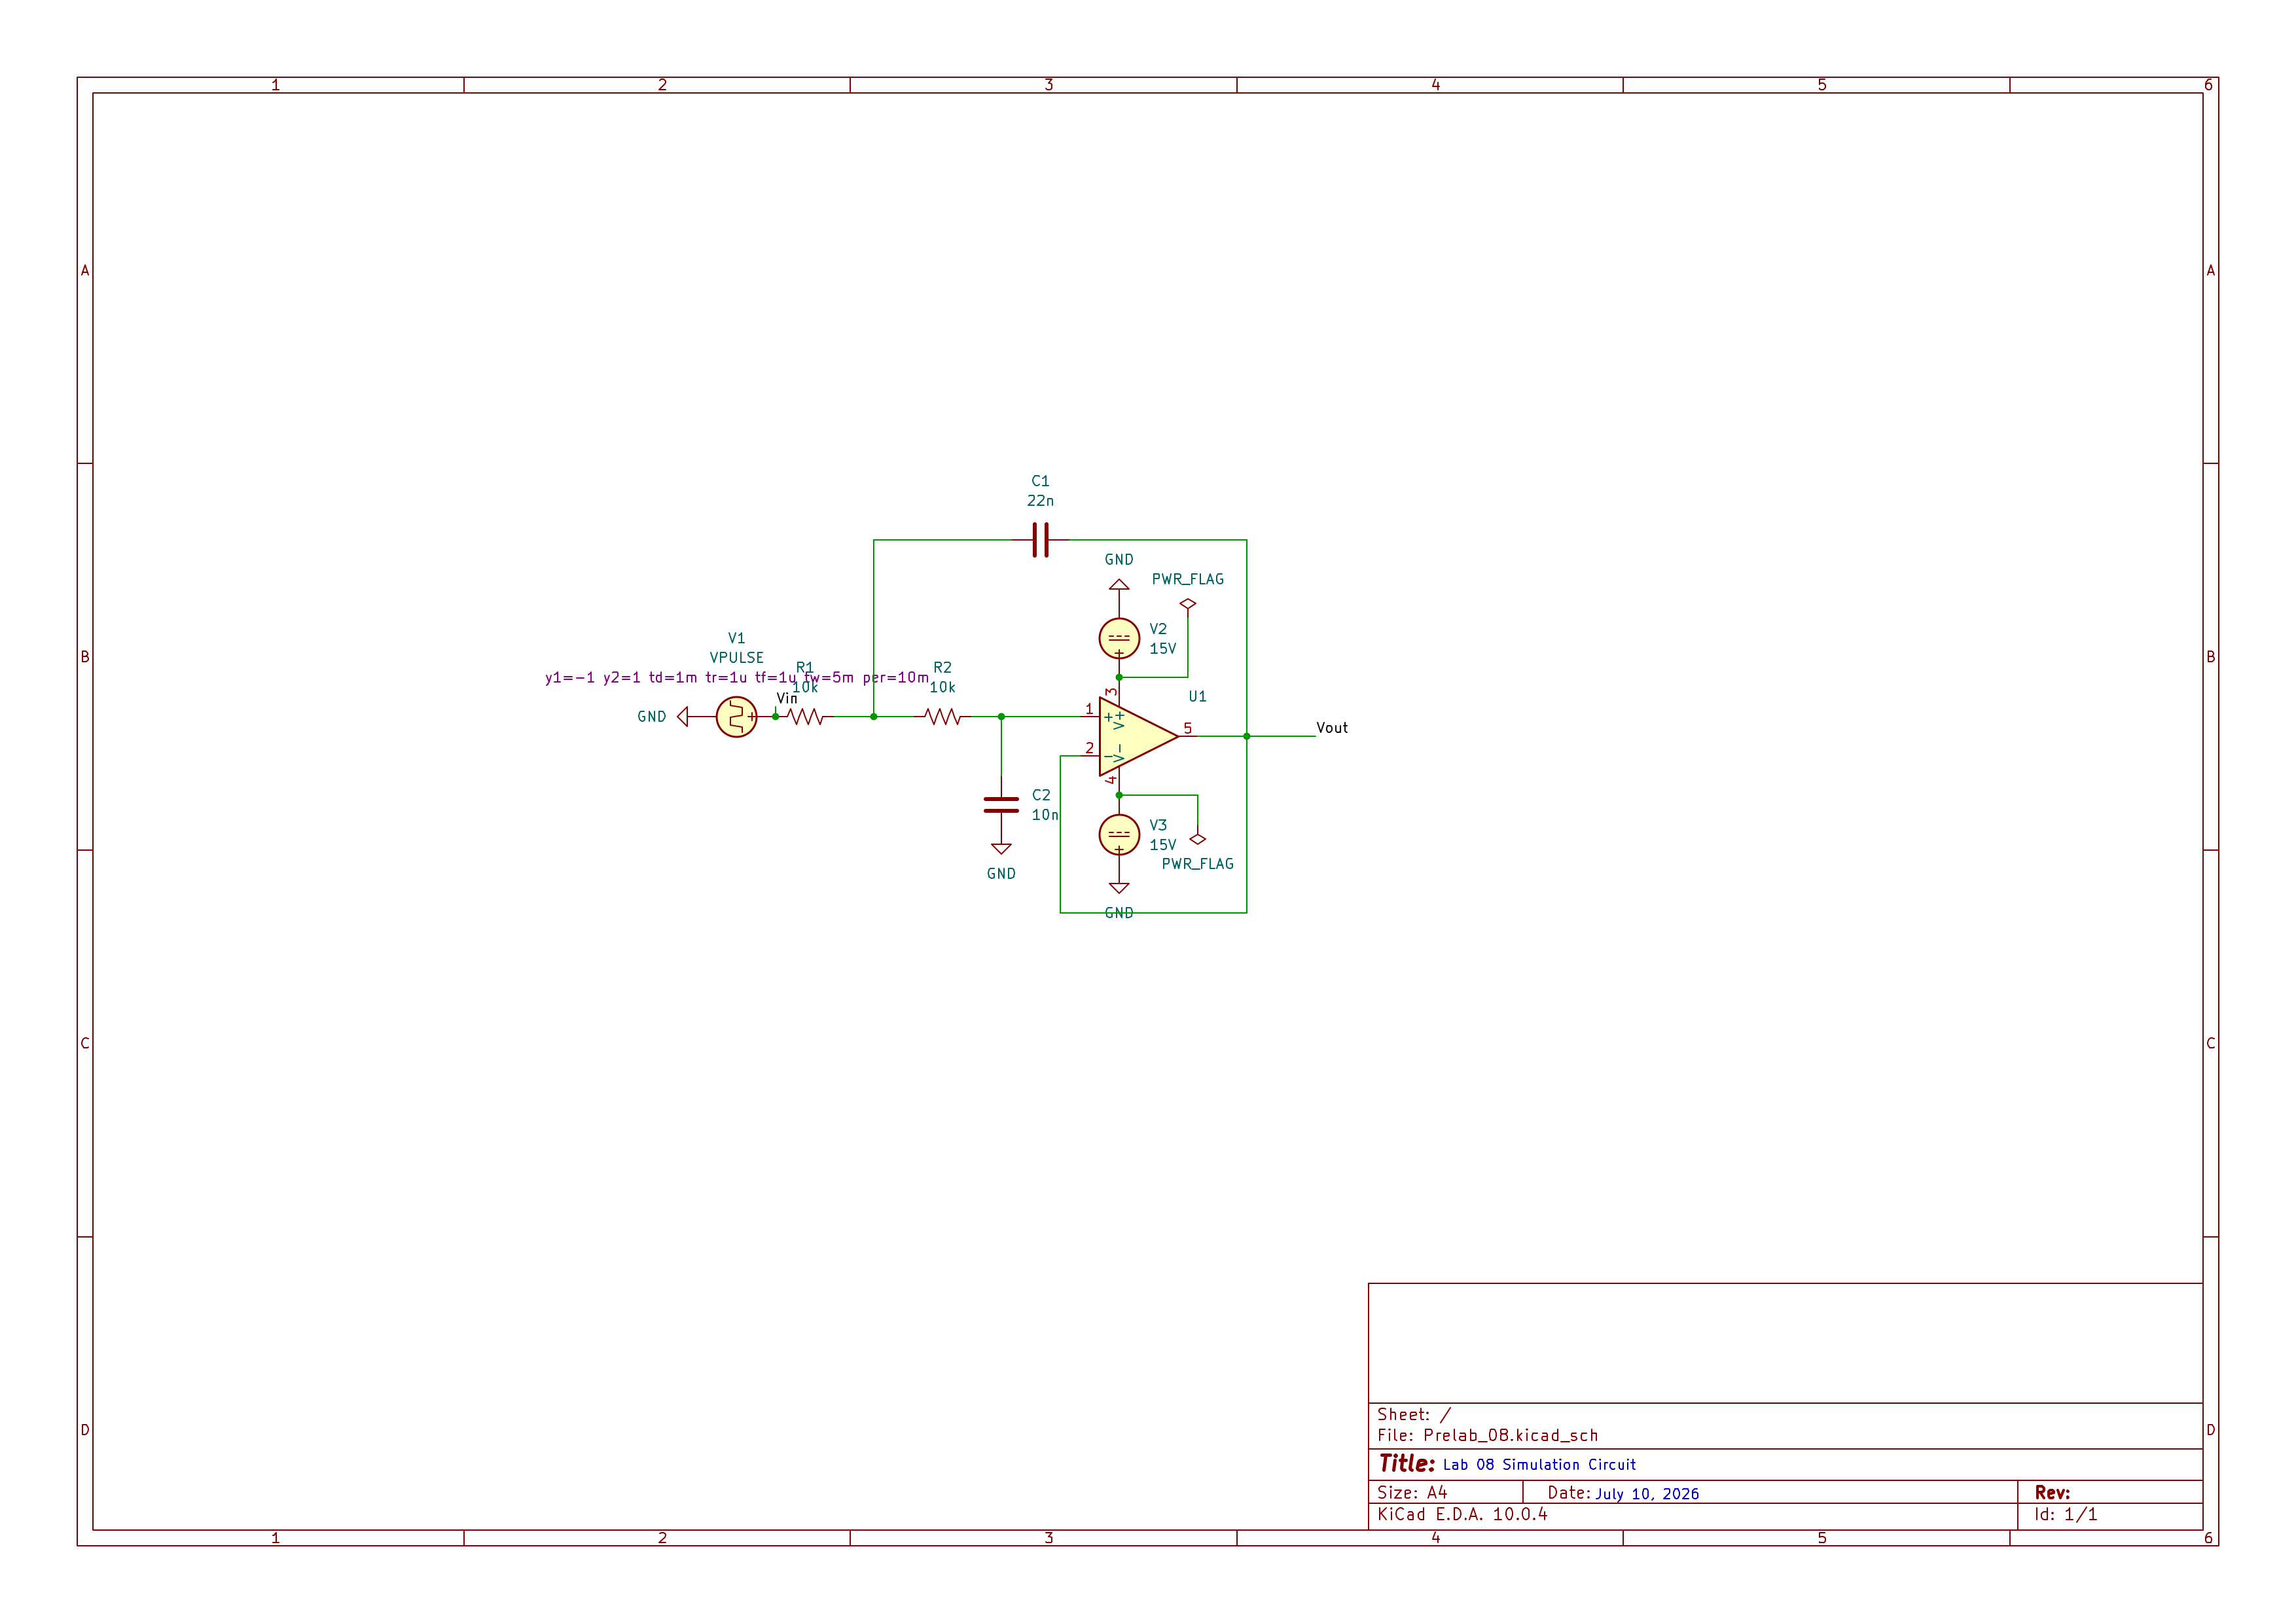
\includegraphics[width=\textwidth]{schematic.png}
    \caption{KiCad schematic used for the transient-response simulations. The
    component values shown correspond to the underdamped case.}
    \label{fig:simulation-schematic}
\end{figure}

\begin{lstlisting}[style=netlist, caption={Critically damped netlist}]
.title KiCad schematic
.include "C:/Users/Abdon Morales/AppData/Local/Programs/KiCad/10.0/share/kicad/symbols/Simulation_SPICE.sp"
.save all
.probe alli
.probe p(V2)
.probe p(C1)
.probe p(R2)
.probe p(C2)
.probe p(R1)
.probe p(V1)
.probe p(V3)
.probe p(XU1)
.tran 5u 20m 0 1u
V2 Net-_U1-V+_ GND DC 15 
C1 /Vout Net-_C1-Pad2_ 10n
R2 Net-_U1-+_ Net-_C1-Pad2_ 16k
C2 Net-_U1-+_ GND 10n
R1 Net-_C1-Pad2_ /Vin 16k
V1 /Vin GND PULSE( -1 1 1m 1u 1u 5m 10m ) 
V3 GND Net-_U1-V-_ DC 15 
XU1 Net-_U1-+_ /Vout Net-_U1-V+_ Net-_U1-V-_ /Vout kicad_builtin_opamp
.end
\end{lstlisting}

\begin{figure}[H]
    \centering
    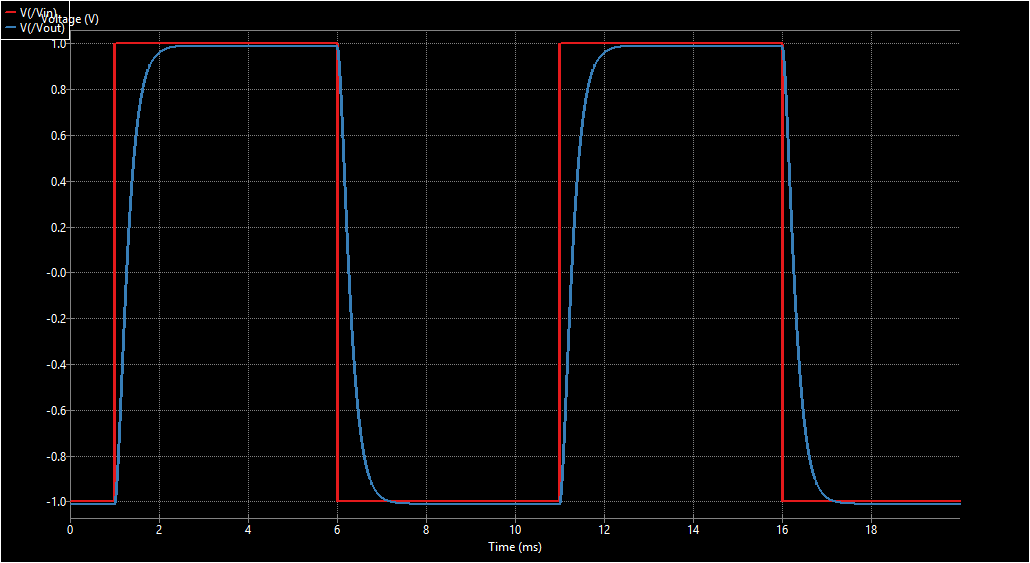
\includegraphics[width=0.8\textwidth]{Prelab_08-criticallyDamped.png}
    \caption{Simulated transient response, critically damped case.}
\end{figure}

\begin{lstlisting}[style=netlist, caption={Overdamped netlist}]
.title KiCad schematic
.include "C:/Users/Abdon Morales/AppData/Local/Programs/KiCad/10.0/share/kicad/symbols/Simulation_SPICE.sp"
.save all
.probe alli
.probe p(V2)
.probe p(C1)
.probe p(R2)
.probe p(C2)
.probe p(R1)
.probe p(V1)
.probe p(V3)
.probe p(XU1)
.tran 5u 20m 0 1u
V2 Net-_U1-V+_ GND DC 15 
C1 /Vout Net-_C1-Pad2_ 10n
R2 Net-_U1-+_ Net-_C1-Pad2_ 5.6k
C2 Net-_U1-+_ GND 10n
R1 Net-_C1-Pad2_ /Vin 47k
V1 /Vin GND PULSE( -1 1 1m 1u 1u 5m 10m ) 
V3 GND Net-_U1-V-_ DC 15 
XU1 Net-_U1-+_ /Vout Net-_U1-V+_ Net-_U1-V-_ /Vout kicad_builtin_opamp
.end
\end{lstlisting}

\begin{figure}[H]
    \centering
    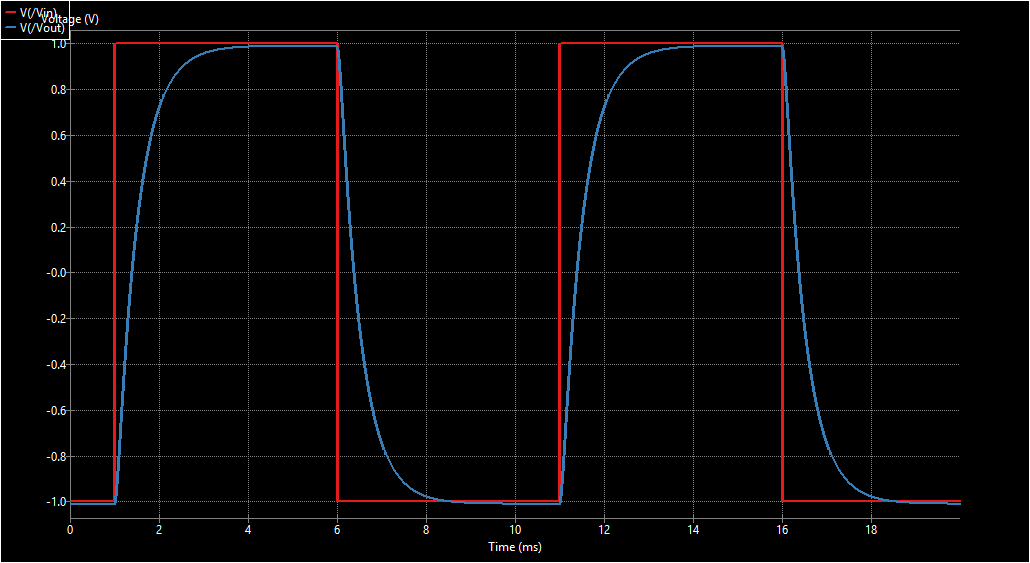
\includegraphics[width=0.8\textwidth]{Prelab_08-overdamped.png}
    \caption{Simulated transient response, overdamped case.}
\end{figure}

\begin{lstlisting}[style=netlist, caption={Underdamped netlist}]
.title KiCad schematic
.include "C:/Users/Abdon Morales/AppData/Local/Programs/KiCad/10.0/share/kicad/symbols/Simulation_SPICE.sp"
.save all
.probe alli
.probe p(V2)
.probe p(C1)
.probe p(R2)
.probe p(C2)
.probe p(R1)
.probe p(V1)
.probe p(V3)
.probe p(XU1)
.tran 5u 20m 0 1u
V2 Net-_U1-V+_ GND DC 15 
C1 /Vout Net-_C1-Pad2_ 22n
R2 Net-_U1-+_ Net-_C1-Pad2_ 10k
C2 Net-_U1-+_ GND 10n
R1 Net-_C1-Pad2_ /Vin 10k
V1 /Vin GND PULSE( -1 1 1m 1u 1u 5m 10m ) 
V3 GND Net-_U1-V-_ DC 15 
XU1 Net-_U1-+_ /Vout Net-_U1-V+_ Net-_U1-V-_ /Vout kicad_builtin_opamp
.end
\end{lstlisting}

\begin{figure}[H]
    \centering
    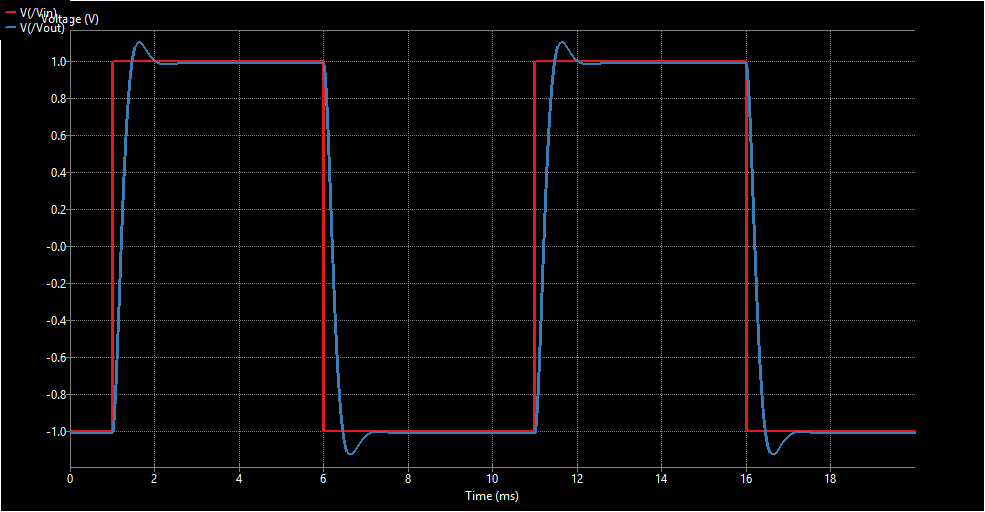
\includegraphics[width=0.8\textwidth]{Prelab_08-underdamped.png}
    \caption{Simulated transient response, underdamped case.}
\end{figure}

%------------------------------------------------------------------------------
\section*{Measurements}

We built the three circuits on the XK700 trainer and captured the input on CH1
and the output on CH2 for each. Several of the resistor and capacitor values from
our prelab design were not stocked in the lab kit, so we substituted the nearest
available parts. This shifted the built values away from the design and, for the
middle case, moved it out of the critically damped regime. Table~\ref{tab:asbuilt}
lists what we actually built and the response those parts produce, computed the
same way as in the Calculations section.

\begin{table}[H]
    \centering
    \caption{As-built component values and the response they produce. $C_1$ is the
    feedback capacitor and $C_2$ the grounded capacitor.}
    \label{tab:asbuilt}
    \begin{tabular}{lcccccl}
        \toprule
        Case (as built) & $R_1$ & $R_2$ & $C_1$ & $C_2$ & $Q$ & Behavior \\
        \midrule
        Overdamped            & \SI{10}{\kilo\ohm} & \SI{10}{\kilo\ohm} & \SI{10}{\nano\farad} & \SI{22}{\nano\farad} & 0.34 & no overshoot \\
        ``Critically damped'' & \SI{10}{\kilo\ohm} & \SI{10}{\kilo\ohm} & \SI{33}{\nano\farad} & \SI{10}{\nano\farad} & 0.91 & rings, $\approx$13\% overshoot \\
        Underdamped           & \SI{10}{\kilo\ohm} & \SI{10}{\kilo\ohm} & \SI{47}{\nano\farad} & \SI{4.7}{\nano\farad} & 1.58 & $\approx$35\% overshoot \\
        \bottomrule
    \end{tabular}
\end{table}

The kit did not have a matched pair of capacitors in the right range for the middle
circuit, so instead of two equal capacitors, which this topology needs for a true
critical response, we used \SI{33}{\nano\farad} and \SI{10}{\nano\farad}. That gives
$Q \approx 0.91$, so the circuit rings slightly rather than sitting on the critical
boundary. We report it here as built and treat it as a lightly underdamped case.

All three captures used a timebase of \SI{5}{\milli\second} per division,
\SI{1}{\volt} per division on CH1, and \SI{2}{\volt} per division on CH2, with the
\SI{100}{\hertz} square-wave input. The output of every circuit follows the input at
unity gain and settles to the input level between edges. Because the sweep was set
to show several full cycles, the transient at each edge is compressed into a small
fraction of a division, so the overshoot and ringing appear only as a spike at each
transition and could not be measured precisely. The overdamped circuit has the
smoothest edges and the \SI{47}{\nano\farad} circuit shows the largest overshoot,
which follows the $Q$ ordering in Table~\ref{tab:asbuilt}.

\begin{figure}[H]
    \centering
    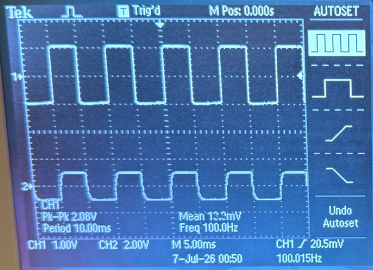
\includegraphics[width=0.8\textwidth]{meas_underdamped.png}
    \caption{Measured response, overdamped case as built
    ($C_1=\SI{10}{\nano\farad}$, $C_2=\SI{22}{\nano\farad}$). CH1 is the input and
    CH2 the output; timebase \SI{5}{\milli\second} per division.}
\end{figure}

\begin{figure}[H]
    \centering
    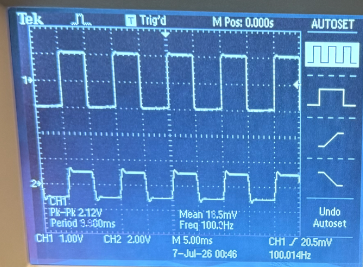
\includegraphics[width=0.8\textwidth]{meas_critical.png}
    \caption{Measured response, as-built ``critically damped'' case
    ($C_1=\SI{33}{\nano\farad}$, $C_2=\SI{10}{\nano\farad}$, $Q\approx0.91$). The
    small overshoot at each edge shows it is lightly underdamped rather than
    critical.}
\end{figure}

\begin{figure}[H]
    \centering
    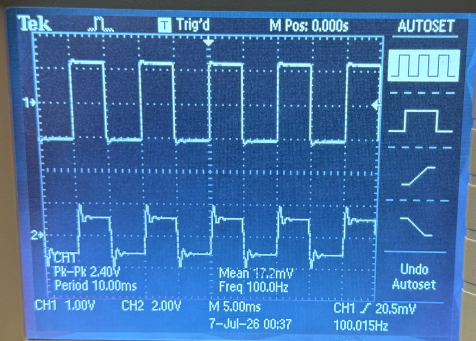
\includegraphics[width=0.8\textwidth]{meas_overdamped.png}
    \caption{Measured response, underdamped case as built
    ($C_1=\SI{47}{\nano\farad}$, $C_2=\SI{4.7}{\nano\farad}$).}
\end{figure}

%------------------------------------------------------------------------------
\section*{Observations \& Discussion}

The measured outputs behaved the way the as-built component values predict. The
overdamped circuit climbed to its final value with no overshoot, the underdamped
circuit overshot and rang before settling, and the middle circuit showed a small
overshoot. That middle circuit was meant to be critically damped, but the lab kit
did not stock a matched pair of capacitors in the range we needed, so we built it
with \SI{33}{\nano\farad} and \SI{10}{\nano\farad} instead of two equal
capacitors. Those unequal values put it at $Q \approx 0.91$, which is lightly
underdamped rather than critical, which is why it rings a little instead of rising
flat. The simulation traces still match the hand-solved responses closely, since
the ideal op-amp model in the simulation has none of the limitations of the real
741.

The biggest limit on the measured comparison was the oscilloscope timebase. We
captured at \SI{5}{\milli\second} per division so several full cycles of the
\SI{100}{\hertz} square wave were on screen, but the second-order transient at each
edge lasts under a millisecond, which is less than a quarter of one division. The
overshoot and ringing were therefore squeezed into a narrow spike at each
transition, and we could not read the ring frequency, peak time, or settling time
from these captures. A faster sweep triggered on a single edge would have spread
the transient across the screen and made those quantities measurable.

Beyond that, the built circuits differ from the designed ones because of the
substituted parts, and the rest of the spread comes from component tolerances and
the real op-amp. Since $Q$ and $f_0$ depend on ratios and products of the resistor
and capacitor values, a few percent of tolerance shifts both. The 741 also has a
finite gain-bandwidth product and a limited slew rate, so it cannot follow the fast
input edges instantly, which rounds the corners of the response compared with the
ideal op-amp used in simulation. Breadboard parasitics and scope-probe loading add
smaller shifts.

If we did this again, the first change would be to capture each transient on a
faster sweep triggered on a single rising edge, around
\SIrange{100}{250}{\micro\second} per division, so the overshoot and ringing fill the screen
and can be measured. We would also source a matched pair of capacitors for the
critical case so it is actually critically damped, and measure each resistor and
capacitor with the LCR meter before building so the theory is based on the parts
actually used. Using 1\% resistors and film capacitors would tighten the spread
further, and replacing the 741 with a faster op-amp would remove most of the edge
rounding on the underdamped cases.

%==============================================================================
\end{document}